\documentclass{article}
\usepackage{graphicx} % Required for inserting images
%Tarih Ekleme

\usepackage[ddmmyyyy]{datetime}
\renewcommand{\dateseparator}{.}
\graphicspath{ {./} }

\usepackage[
  backend=bibtex,
  style=chem-angew,
  citestyle=numeric-comp,
  sorting=none,  
]{biblatex}
\addbibresource{kaynakca.bib}
\usepackage{pgf-pie}
\usepackage[utf8]{inputenc}
\usepackage{array}
\usepackage{tikz}
\usetikzlibrary{positioning}
\usetikzlibrary{shapes,arrows,arrows,positioning,fit}
\usetikzlibrary{shapes,arrows}



\title{Yapay Zeka ile Malware Tespiti
Final Raporu}
\author{Mustafa Akbaba}
\date{June 2024}

\begin{document}

\begin{figure}
    \centering
        \includegraphics{logo-1.jpg}
\end{figure}
\maketitle

\begin{abstract}
\noindent Bu Projede makine öğremi ve statik analiz yöntemlerini kullanarak malware tespiti amaçlanmıştır. Kullanılan veri seti ile PE dosyalarını analiz ederek iyi huylu mu kötü huylumu olduğuna karar verir.
\end{abstract}

\section{Giriş}
İnternetin hızla gelişmesiyle birlikte kötü amaçlı yazılımlar günümüzde en büyük  siber tehditlerden biri haline geldi.Bilgi çalma, casusluk vb. dahil olmak üzere kötü amaçlı eylemler gerçekleştiren herhangi bir yazılım, kötü amaçlı yazılım olarak adlandırılabilir. \\
Kötü amaçlı yazılımların çeşitliliği artarken, anti-virüs tarayıcıları koruma ihtiyaçlarını karşılayamamakta ve milyonlarca ana bilgisayarın saldırıya uğramasına neden olmaktadır. Kaspersky Labs'a (2023) göre\cite{kasper}, 2023'te Kaspersky'nin sistemleri toplamda yaklaşık 125 milyon zararlı dosya tespit etti. Windows, siber saldırılar için birincil hedef olmaya devam etti ve günlük olarak tespit edilen tüm kötü amaçlı yazılım dolu verilerin yüzde 88'ini oluşturdu. Çeşitli komut dosyaları ve farklı belge formatları aracılığıyla yayılan kötü amaçlı dosyalar, günlük olarak tespit edilen tüm kötü amaçlı dosyaların yüzde 10'unu oluşturarak ilk üç tehdit arasında yer aldı.

\section{Literatür Araştırması}
Sınıflandırma Algoritması kullanımında Machine Learning approach for Malware Detection(2016) projesinden yardım alınmıştır .\cite{git1}Bu yaklaşım, sonuçlarını karşılaştırarak tahmin için hangisinin kullanılacağına karar vermeden önce 6 farklı sınıflandırma algoritmasını dener.
\\
Yapay zekayı kod içinde nasıl kullanılıacağını anlamak için Malware Detection by Machine Learning and Deep Learning(2021) projesinden yardım  alınmıştır.\cite{ytp1}Bu çalışmada kötü amaçlı yazlım tespiti için machine learning ve deep learning yöntemleri kullanılmıştır.
 \\
 Android Malware Detection Using Machine Learning(2022) projesinde konuyu daha iyi kavramak açısından incelemek için kullanılmıştır.\cite{git2}Bu projede, Android kötü amaçlı yazılım tespit sorununu çözmeye yönelik farklı yaklaşımlar sunulmakta ve gösterilmektedir.Bu, makine öğrenimi modelleri aracılığıyla elde edilir. En Önemli Makine Öğrenimi algoritmaları andorid haritalama veri kümelerine uygulanır ve ardından android uygulamasının kötü amaçlı yazılım içerip içermediğini tespit etmemizi sağlar.

 \section{Veri Seti}
\subsection{Ağ Trafiği Analizi}
Bu veri seti  içeriği ağ trafiği analizi için tipik özellikleri içeriyor. Bu tür veri setleri genellikle ağ trafiği analizi, siber güvenlik tehditlerinin tespiti ve ağ performansı optimizasyonu gibi alanlarda kullanılır.\\
Veri setinizdeki sütunların içeriği
\begin{itemize}
    \item Kaynak ve hedef IP adresleri ve bağlantı noktaları
    \item İletim protokolü
    \item Zaman damgaları
    \item İletim süreleri ve paket sayıları
    \item İletim ve alım yönünde paket boyutları
    \item İletim ve alım yönünde sürelerin istatistikleri
    \item TCP kontrol bayrakları (FIN, SYN, RST, vb.)
    \item Aktivite ve boşta kalma süreleri
\end{itemize}
Veri setindeki özelliklerin istatistiksel analizi, kötü amaçlı trafiği tanımlamak için tipik örüntülerin belirlenmesine yardımcı olabilir. Örneğin, belirli bir kaynak portundan gelen çok sayıda bağlantı veya belirli bir hedefe yönlendirilen anormal büyüklükteki veri paketleri gibi belirgin örüntüler, potansiyel olarak zararlı trafiği işaret edebilir.\cite{1}
\subsection{Bellek Analizi}
Bu veri seti, bir tür sistem izleme veya güvenlik taraması sonucu elde edilmiş. Her bir özellik, farklı sistem bileşenleri veya davranışlarının belirli özelliklerini temsil ediyor.


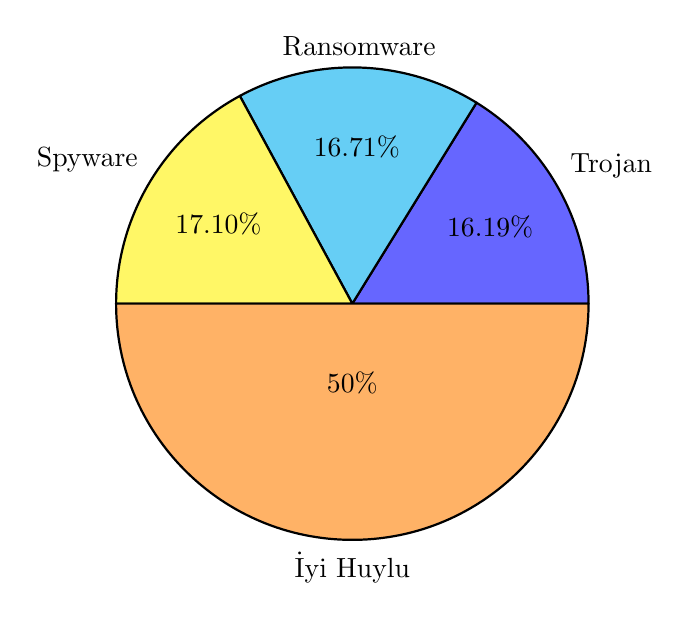
\begin{tikzpicture}
\pie{16.19/Trojan, 16.71/Ransomware, 17.10/Spyware, 50/İyi Huylu}
\end{tikzpicture}

Genel olarak, veri seti, bilgisayar sistemlerindeki işlemler, DLL'ler, tanıtıcılar, modüller, hizmetler ve geri aramalar gibi çeşitli bileşenlerin özelliklerini içeriyor.Bu veri seti, bilgisayar sistemlerindeki çeşitli bileşenlerin özelliklerini içerir ve bu özellikler, potansiyel olarak zararlı faaliyetlerin belirlenmesinde ve güvenlik tehditlerinin sınıflandırılmasında kullanılabilir. Örneğin, işlem sayısı, işlem başına tanıtıcı sayısı, DLL sayısı gibi özellikler, sistemin normal veya anormal davranışlarını tanımlamak için kullanılabilir.\cite{c}
\section{Yöntem}
Kötü amaçlı yazılım tespit teknikleri imza tabanlı ve davranış tabanlı yöntemler olarak ikiye ayrılır. Bu yöntemlere geçmeden önce, kötü amaçlı yazılım analizi için kullanılan yaklaşımının temellerini anlamak önemlidir: statik ve dinamik kötü amaçlı yazılım analizi. Adından da anlaşılacağı üzere, statik analiz "statik olarak", yani dosya yürütülmeden gerçekleştirilir. Buna karşılık, dinamik analiz, dosya yürütülürken, örneğin sanal makinede  gerçekleştirilir.
\begin{enumerate}
\item İmza Tabanlı Kötü Amaçlı Yazılım Tespiti
Kötü amaçlı yazılımları tanımlamak için virüs kodlarını/hash'lerini kullanır. Kötü amaçlı yazılım, onu tanımlamak için kullanılan benzersiz bir kod taşır. Bir dosya bilgisayara ulaştığında, kötü amaçlı yazılım tarayıcısı kodu toplar ve bulut tabanlı bir veritabanına gönderir. Veritabanı geniş bir virüs kodu koleksiyonuna sahiptir. Dosya kodu listede bulunursa, veritabanı dosyanın kötü amaçlı yazılım olduğuna dair bir karar verir. Anti-malware dosyayı bilgisayardan reddeder ve siler. Yeni bir kötü amaçlı yazılım keşfedilirse, kodu listeye eklenir.
,,
\begin{itemize}
\item Artıları:
 Bu analizi yöntemi, internette yayılan popüler olan kötü amaçlı yazılım türleri söz konusu olduğunda en hızlı ve en doğru yöntemdir.
\item Eksileri:
Popüler olmayan kötü amaçlı yazılımlar söz konusu olduğunda en doğru yöntem değildir. Doğruluğu kullandığı veri setine bağlıdır.
\end{itemize}
\item Davranış Temelli Kötü Amaçlı Yazılım Tespiti
Kötü amaçlı yazılımları davranışa dayalı olarak tanımlayarak adının hakkını verir. Kötü amaçlı yazılımlar genellikle yasal yazılımlardan farklı davranır. Kötü amaçlı yazılım kendini çalıştırmadan önce bile antivirüs ürünlerine kimliğini açıklayabilecek davranışlar sergileyebilir. Davranış tabanlı tespit, bir yazılımın kötü amaçlı olup olmadığını belirlemek için bu davranışların taranmasını içerir\cite{met1}.
\begin{itemize}
\item Artıları:
Popüler olmayan kötü amaçlı yazılımlar için en iyi sonucu verir.
\item Eksileri:
Taramaya gerek kalmadan mümkün olan en kısa sürede kaldırılması gereken kötü amaçlı yazılımları durdurma yeteneğinden yoksundur.
\end{itemize}
\end{enumerate}
\subsection{Makine Öğrenimi ve Derin Öğrenme }
\subsubsection{Makine Öğrenimi}
Makine öğrenmesi, çeşitli algoritmik teknikler kullanılarak farklı makine öğrenmesi modelleri türlerinden oluşur. Verilerin niteliğine ve istenilen sonuca bağlı olarak üç öğrenme modelinden biri kullanılabilir: 
\begin{itemize}
    \item Denetimli:
    \\Denetimli öğrenmede bağımsız değişkenlerin işaret ettiği bağımlı değişkenin varlığından bahsettiğimiz, bağımsız değişkenleri eğiterek buradan çıkan sonuca referans veren bir yöntemdir.
    \item Denetimsiz:
    \\Denetimsiz öğrenmede, algoritma verilerin kendisinin kullanıldığı anlamlı sonuçlar bulmaya çalışır. Sonuç, örneğin, her kümede ilişkilendirilebilecek bir dizi veri noktası kümesi olabilir. Kümeler örtüşmediğinde daha iyi sonuç verir. Birbirine benzer verileri aynı küme altında gruplara ayırır.
    \item Yarı Denetimli
\end{itemize}
Bu modellerin her birinde, kullanılan veri kümelerine ve amaçlanan sonuçlara göre bir veya daha fazla algoritmik teknik uygulanabilir. Makine öğrenmesi algoritmaları temel olarak olayları sınıflandırmak, örnekler bulmak, sonuçları tahmin etmek ve bilinçli kararlar vermek için tasarlanmıştır. Algoritmalar karmaşık ve daha öngörülemeyen veriler söz konusu olduğunda mümkün olan en iyi doğruluğu elde etmek için tek seferde bir veya bir arada kullanılabilir\cite{ml}.
\subsubsection{Yaygın Makine Öğrenim Algoritmaları}
\begin{itemize}
    \item Random Forests, (sınıflandırma ve regresyon için)
    \item Linear regression, en küçük kareler yöntemi(sayısal veriler için),
    \item Logistic regression (ikili sınıflandırma için)
    \item Karar ağaçları (sınıflandırma ve regresyon için)
\end{itemize}
\subsection{Feature Engineering}
Feature engineering (Özellik Mühendisliği), ham verileri seçme, değiştirme ve denetimli öğrenmede kullanılabilecek özelliklere dönüştürme ve veriyi makine öğrenmesi modellerine hazırlama sürecidir. Feature(Özellik), tahmine dayalı bir modelde kullanılabilecek herhangi bir ölçülebilir girdidir. Doğru olarak işletildiğinde modellerin tahmin gücünün artmasına yardımcı olur\cite{FE}.
\subsubsection{Encoding}
 Bazı makine öğrenmesi algoritmaları kategorik veriler üzerinde çalışamadığı için sayısal verilere veya vektörlere dönüşmesi gerekmektedir. One hot encoding ve label encoding olarak yöntemleri mevcuttur.
 \subsubsection{Correlation}
 Korelasyon analizi; değişkenler arasındaki ilişki, bu ilişkinin yönü ve şiddeti ile ilgili bilgiler sağlayan istatiksel bir yöntemdir.
 Korelasyon katsayısı, bağımlı değişken ile bağımsız değişkenler arasındaki ilişkinin gücünü gösteren bir katsayıdır. Örneğin; öğrencinin ders çalışma süresi ile aldığı istatistik notu arasında ilişki olup olmadığını veya borsada işlem gören bir hisse senedinin belli bir dönemdeki günlük getirisi (X) ile içinde yer aldığı bir endeksin günlük getirisi (Y) arasındaki ilişki korelasyon katsayısı ile incelenebilir. Korelasyon katsayısı değişkenlerin yönü ve etkileşimlerin nasıl olduğu hakkında bilgi verir\cite{KA}.
 \begin{center}
\begin{tabular}{ | m{5em} | m{1cm}| m{1cm} | } 
  \hline
 Korelasyon Aralığı& İlişki Düzeyi \\ 
  \hline
  (-0,25)-00 ve 0,00-0,25 & Çok Zayıf\\ 
  \hline
 (-0,49)- (-0,26) ve 0,26-0,49 & Zayıf \\ 
  \hline
  (-0,69)-(-0,50) ve 0,50-0,69 & Orta\\ 
  \hline
  (-0,89)-(-0,70) ve 0,70-0,89 & Yüksek\\ 
  \hline
   (-1,00)-(-0,90) ve 0,90-1,00 & Çok Yüksek\\ 
  \hline
\end{tabular}
\end{center}

\subsection{Methodlar}
\subsubsection{StandartScaler}
Standardscaler, veri setinin her bir öznitelik değerinin ortalaması sıfır ve standart sapması bir olacak şekilde yeniden ölçeklendirilmesi işlemidir. Bu işlem, veri setindeki özniteliklerin farklı ölçeklerde olması durumunda, öğrenme algoritmalarının doğru bir şekilde çalışmasına olanak tanır.

Standardscaler, verilerin daha tutarlı bir şekilde işlenmesine olanak tanır ve makine öğrenmesi modellerinin daha iyi performans göstermesini sağlar. Özellikle, çok sayıda öznitelik içeren veri setlerinde, Standardscaler kullanımı önemlidir\cite{SS}

\subsubsection{.fit()}
Bu methodu veri setinde dönüşüm yapılacağında, label encoding yapılacağında veya bir model kurulacağında kullanırız. Bu yöntemlerden her birini uygulamak için bazı parametreler gerekir. Örnek vermek gerekirse eğer bir modelde kullanacaksak veri setinin μ (ortalama), σ (standart sapma) değerlerine ihtiyaç vardır. Başka bir örnek, eğer veri setini 0 ile 1 arasında bir normalizasyon işlemi yapılacaksa veri setindeki minimum ve maksimum değerler gerekir. .fit() methodu bu parametleri arka planda hesaplar ancak bu parametrelerle bir işlem yapmaz. Yani bu methodun kendi başına bir çıktısı yoktur.

\subsubsection{.transform()}
Bu method adından da anlaşılacağı gibi dönüşüm işlemini gerçekleştirir. Ancak bir veri setini fit etmeden transform işlemi uygulanamaz çünkü dönüşüm yapılırken kullanılacak olan parametreler hesaplanmamıştır\cite{Method}.

\subsection{Algoritmalar}
\subsubsection{Decision Tree}
Decision tree algoritması, basitliği ve yorumlanabilirliği nedeniyle sınıflandırma görevleri için popülerdir. Verileri farklı niteliklere göre alt kümelere bölerek ve ağaç benzeri bir karar modeli oluşturarak çalışır. Algoritma, örnekleri sınıflandırmak için if-else koşullarının hiyerarşik yapısını kullanır. Decision tree, finans, sağlık ve pazarlama gibi çeşitli alanlarda yaygın olarak kullanılmaktadır.
\subsubsection{ Random Forest}
Random forest, tahminlerin doğruluğunu artırmak için birden fazla karar ağacını birleştiren bir toplu öğrenme yöntemidir. Birçok karar ağacı oluşturarak ve çıktılarını oylama yoluyla toplayarak çalışır. Ormandaki her karar ağacı, eğitim verilerinin rastgele bir alt kümesi ve girdi özelliklerinin rastgele bir alt kümesi kullanılarak oluşturulur. Random Forest, sağlamlığı ve yüksek boyutlu özelliklerle büyük veri kümelerini işleme yeteneği ile bilinir.
\subsubsection{ Support Vector Machines}
SVM, sınıflandırma ve regresyon görevleri için güçlü bir algoritmadır. SVM, sınıfları maksimum düzeyde ayıran yüksek boyutlu bir uzayda optimal bir hiper düzlem bulur. Girdi verilerini daha yüksek boyutlu bir öznitelik uzayına dönüştürür ve en büyük kenar boşluğuna sahip optimum ayırıcı hiper düzlemi bulur. SVM'ler görüntü tanıma, metin sınıflandırma ve biyoinformatikte yaygın olarak kullanılır.
\subsubsection{K-Nearest Neighbors (KNN)}
KNN, sınıflandırma için kullanılan parametrik olmayan ve tembel bir öğrenme yöntemidir. Örnekleri, eğitim verilerindeki k en yakın komşuya olan yakınlıklarına göre sınıflandırır. KNN basit ama etkilidir ve temel veri dağılımı hakkında herhangi bir varsayımda bulunmaz. Genellikle tavsiye sistemlerinde, anormallik tespitinde ve örüntü tanımada kullanılır.
\subsubsection{Gradient Boosting }
XGBoost ve LightGBM gibi Gradient Boosting algoritmaları, zayıf öğrenicileri birleştirerek güçlü bir tahmine dayalı model oluşturan toplu öğrenme yöntemleridir. Önceki modellerin yaptığı hataları düzelten modelleri sırayla ekleyerek iteratif olarak çalışırlar. Gradient Boosting algoritmaları, web arama sıralaması, kredi riski analizi ve dolandırıcılık tespiti dahil olmak üzere çeşitli alanlarda mükemmeldir.

\subsection{Model Performan Değerlendirmesi}
\subsubsection{Doğruluk (Accuracy)}
Modelin doğru tahmin ettiği örneklerin oranıdır. Doğruluğun maksimum değeri 1 olabilir. Örneğin, 100 örneğin 80'inin doğru sınıflandırıldığı bir modelin doğruluk skoru 0.8 olacaktır.\\
Formül:\\

Doğruluk = (TP + TN) / (TP + TN + FP + FN)
\subsubsection{Hassasiyet (Precision)}
Pozitif olarak sınıflandırılan örneklerin ne kadarının gerçekten pozitif olduğunu gösterir. Hassasiyet modelin pozitif sınıfı doğru sınıflandırma yeteneğini ölçmektedir. Aşağıdaki formülden de anlaşılacağı üzere hassasiyet pozitif olarak doğru bilinen tahminlerin tüm pozitif tahminlere oranı olarak ifade edilebilir.\\
Formül:\\
Hassasiyet = TP / (TP + FP)
\subsubsection{Duyarlılık (Recall)}
 Gerçek pozitif örneklerin ne kadarının pozitif olarak sınıflandırıldığını gösterir. Aşağıdaki formül incelendiğinde duyarlılık, pozitif olarak doğru tahmin edilenlerin gerçek pozitiflere oranı olarak ifade edilebilir.\\
 Formül:\\
 Duyarlılık = TP / (TP + FN)
 \subsubsection{F1 Skor (F1 Score)}
 F1 Skor ise Hassasiyet (Precision) ve Duyarlılık (Recall) skorlarının harmonik ortalamasıdır.\\
 Formül:\\
 F1 Skor = 2 * ((Precision * Recall) / (Precision + Recall))\cite{P}
 \subsection{Portable Executable}
Portable Executable (kısaca PE), Windows’ un çalıştırılabilir dosya formatıdır. Dosya formatları , programların fonksiyonlarla alakalı bir takım bilgileri analiz yapan kişiye sunabilmektedir. PE dosya formatı Windows executable ve DLL dosyaları tarafından kullanılabilmektedir. PE dosyaları başlık bilgileri ile başlar ve bu başlık bilgileri program için gereken kütüphane fonksiyonlarını uygulama tipleri gibi bilgileri içermektedir.Bağlı kütüphaneler ve fonksiyonlardan yararlanılarak analiz için bilgiler edilebilir. PE dosya 
başlığı program tarafından yüklenen kütüphane ve fonksiyonlar ile alakalı bilgileri tutar.
\cite{PEP}
\subsubsection{File Header}
Bu başlık, PE dosyasına ait önemli birkaç bigiyi tutuyor.
\begin{itemize}
    \item Machine
    \item SizeOfOptionalHeader
    \item Characteristics    
\end{itemize}

\subsubsection{Optional Header}
programın entry pointi, işletim sisteminin versiyonu gibi çok kritik blgiler taşır. Bu kısmın 32 bit ve 64 bit versiyonları var fakat sadece boyut olarak farklılıklar barındırıyor.
\begin{itemize}
    \item  MajorLinkerVersion
    \item MinorLinkerVersion
    \item SizeOfCode
    \item SizeOfInitializedData 
\end{itemize}

\subsubsection{Section}
PE dosyası sectionlardan oluşur. Bu sectionlar içindeki verinin nasıl bir yapıda olduğunu belirtir.Sadece global ve statik veriler section'larda saklanıyor. Lokal değişkenler .data, .bss gibi section'larda saklanmıyor. Bunun yerine ptogramı execute ettiğimizde çalışma zamanında oluşturulup stack te depolanır ve gerektiğinde stack'ten okunup gerekli işlem yapılır.

\subsubsection{File Import}
Bildiğiniz üzere yazılan programlarda başka .dll' lerde ki fonksiyonları kullanıyoruz. Bu fonksiyonları kullanabilmek için kullandığımız dll'lerin kayıtlarının PE dosya formatında bir yerde bulunması gerekiyor. Aksi halde bu fonksiyonları kullanamayız. İşte bu kayıtlar ".idata" section'ında yer alıyor. Loader(PE dosyamızı rame map eden program) .idata section'ındaki bilgileri kullanarak gerekli dll'lerin ve fonksiyonların adreslerini executable image'ye bağlar.
\subsubsection{File Export}
Biz normalde başka .dll'lerin içerisindeki fonksiyonları kullanıyoruz (import), export bunun tam tersi bizim dışarıya kullanılabilecek bir fonksiyon vermemiz denebilir.
\subsubsection{File Resources}
Portable Executable (PE) dosya formatındaki kaynaklar, bir uygulamanın veya yürütülebilir dosyanın içinde bulunan metin, grafik, ses, ikonlar ve diğer öğeleri içeren veri parçacıklarıdır. Bu kaynaklar, bir uygulamanın görsel ve işitsel unsurlarını, dil seçeneklerini, simgelerini ve diğer öğelerini içerir. PE dosya formatında kaynakları temsil etmek için özel bir bölüm vardır ve bu bölüm "RESOURCE" adını taşır.PE dosyalarındaki kaynaklar, çeşitli özelliklere ve türlerde verilere sahip olabilir. Bu kaynaklar, uygulamanın kullanıcı arayüzünü, dil seçeneklerini, ikonlarını, resimlerini, metin kaynaklarını ve daha fazlasını içerebilir. RESOURCE bölümü, kaynakların düzenli bir şekilde depolanmasını sağlar ve uygulamaların bu kaynaklara erişimini kolaylaştırır.
\cite{PE2}

\section{Kod Bölümleri}
\subsection{get entropy}
Shannon entropy, bir veri dizisinin düzensizliğini veya belirsizliğini ölçen bir metriktir. Daha yüksek bir entropi, verinin daha fazla belirsizlik veya düzensizlik içerdiği anlamına gelir.
\begin{itemize}
    \item 0 * 256:
    Bir liste oluşturur ve bu listenin her elemanı 0 olan 256 eleman içerdiği anlamına gelir. 
    \item isinstance(x, int): x değişkeninin bir tamsayı olup olmadığını kontrol eder. 
    \item ord(x): Eğer x bir tamsayı değilse, yani bir karakter (char) ise, ord() fonksiyonu kullanılarak karakterin ASCII değerine dönüştürülür. 
\end{itemize}
\subsection{get resources}
Verilen PE (Portable Executable) dosyasından kaynak bilgilerini (resources) çıkarır. Bu kaynaklar, dosyanın içerdiği gömülü verileri temsil eder.
\subsection{get version info}
PE dosyasının sürüm bilgilerini çıkarır. Dosyanın sürüm numarası, imzası ve diğer özelliklerini içerir.
\subsection{extract info}
 PE dosyasının çeşitli özelliklerini çıkarır. Bu özellikler, dosyanın boyutu, bölümleri, import ve export sayıları, kaynakları ve sürüm bilgilerini içerir.
 \subsection{İçe Aktarım}
 Bir yazılım bileşeninin, kendi kodunda başka bir bileşeni kullanmak için dışarıdan içe aktarmasıdır. Bu, genellikle bir yürütülebilir dosyanın veya bir DLL'nin bir işlevini veya hizmetini kullanmak için diğer bir yürütülebilir dosya veya DLL'yi içe aktarması anlamına gelir. Örneğin, bir programın kullanıcı arayüzü için Windows API işlevlerini kullanması veya bir DLL'nin işlevlerini çağırması, içe aktarımı temsil eder.
 \subsection{Dışa Aktarım}
 Bir yazılım bileşeninin, kendi kodunda bulunan bir işlevi veya hizmeti diğer bileşenlere sunmasıdır. Bu, genellikle bir yürütülebilir dosyanın veya bir DLL'nin, kendi işlevlerini diğer bileşenlerin kullanımına sunması anlamına gelir. Örneğin, bir DLL'nin belirli işlevlerini diğer programlar kullanabilmek için dışa aktarması, dışa aktarımı temsil eder\cite{PE3}\cite{PE4}\cite{PE5}\cite{PE6}\cite{PE7}\cite{PE8}.
 \begin{figure}
 	
 	\tikzstyle{block} = [rectangle, draw, fill=blue!20, 
 	text width=10em, text centered, rounded corners, minimum height=2em]
 	\tikzstyle{line} = [draw, -latex']
 	\tikzstyle{decisionn} = [diamond, draw, fill=yellow!20, 
 	text width=4em, text badly centered, node distance=4cm, inner sep=0pt]
 	\tikzstyle{blockk} = [rectangle, draw, fill=green!20, 
 	text width=8em, text centered, rounded corners, minimum height=2em]
 	\tikzstyle{blockkk} = [rectangle, draw, fill=red!20, 
 	text width=6em, text centered, rounded corners, minimum height=2em]
 	
 	\begin{tikzpicture}[node distance = 2cm, auto]\label{ams1}
 	\node [block] (a) {Veri Setini Eğitme};
  	\node [block, below of=a] (b) {Analiz};
 	\node [block, below of=b] (c) {Özellik Çıkarımı}
        \node [block, below of=c] (d) {Pkl Dosyalarını oluşturma}
 	\node [block, below of =d] (e) {Dedektör};
        \node [decisionn, below right=1.5cm and 1.0cm of e,node distance=2.5cm] (f) {Malware?};
 	\node [block, right of=a, node distance=7.5cm] (g) {Pe Örneği };
 	\node [block, below of=g] (h) {Analiz};
 	\node [block, below of=h] (ı) {Özellik Çıkarımı};
    \node [blockkk, below left=1.5cm and 1.0cm of f,node distance=2.5cm] (j) {Kötü Huylu};
    \node [blockk, below right=1.5cm and 1.0cm of f,node distance=2.5cm] (k) {İyi Huylu};
 	
        \path [line] (a) -- (b);
 	\path [line] (b) -- (c);
        \path [line] (c) -- (d);
 	\path [line] (d) -- (e);
 	\path [line] (e) -- (f);
 	\path [line] (g) -- (h);
 	\path [line] (h) -- (ı); 
 	\path [line] (ı) -- (e);
 	\path [line] (f) -- (j);
 	\path [line] (f) -- (k);
 	
 	\end{tikzpicture}
 	\caption{Kodun Çalışma Mantığı}
 \end{figure}

 \section{Bulgu ve Tartışma}
  

Tablolarda görülen sonuçlar  yapay zeka modelinin farklı parametlerini değiştirerek doğruluk oranı arttırılmıştır. Bu parametreler şunlardır:
\subsection{n Estimators}
n Estimators parametresi, Random Forest ve Gradient Boosting gibi ağaç tabanlı ensemble öğrenme modellerinde kullanılan bir parametredir. Bu parametre, modele dahil edilecek karar ağaçlarının sayısını kontrol eder.\\
n Estimators seçiminde göz önünde bulundurulması gereken bazı faktörler şunlardır:
\begin{itemize}
    \item Veri kümesinin boyutu: Daha büyük veri kümeleri, daha fazla karar ağacına izin verebilir.
    \item Veri kümesinin karmaşıklığı: Daha karmaşık veri kümeleri, daha fazla karar ağacı gerektirebilir.
    \item Modeli kullanılacak görev: Sınıflandırma görevleri, regresyon görevlerinden daha fazla karar ağacı gerektirebilir.
\end{itemize}
n Estimators'ın bazı yaygın değerleri şunlardır:
\begin{itemize}
    \item 100: Bu, birçok uygulama için iyi bir başlangıç noktasıdır.
     \item 1000: Bu, daha karmaşık veri kümeleri için daha uygundur.
     \item 10000: Bu, çok karmaşık veri kümeleri için kullanılabilir.
\end{itemize}

\subsection{max depth}
max depth, karar ağaçları ve rastgele ormanlar gibi ensemble öğrenme modellerinde kullanılan bir hiperparametredir. Bu parametre, bir karar ağacının veya alt ağacın maksimum derinliğini kontrol eder. Derinlik, bir düğümden kök düğüme giden en uzun yol uzunluğu ile ölçülür.\\
max depth'in bazı yaygın değerleri şunlardır:
\begin{itemize}
    \item 2: Bu, birçok uygulama için iyi bir başlangıç noktasıdır.
    \item 5: Bu, daha karmaşık veri kümeleri için daha uygundur.
     \item 10: Bu, çok karmaşık veri kümeleri için kullanılabilir.
\end{itemize}
    
\subsection{n jobs}
n jobs, Python'daki joblib kütüphanesi tarafından kullanılan bir parametredir. Bu parametre, birden fazla CPU çekirdeği veya işlemciyi kullanarak kodun paralel olarak yürütülmesine izin verir.\\
n jobs'u kullanmanın faydaları:
\begin{itemize}
    \item Hesaplama süresini önemli ölçüde kısaltabilir. Özellikle büyük veri kümeleri üzerinde çalışırken, paralel işleme önemli bir hız artışı sağlayabilir.
    \item Bilgisayarınızın kaynaklarını daha verimli kullanabilirsiniz. n jobs, tüm işlemci çekirdeklerinizi kullanarak kodunuzu çalıştırarak bilgisayarınızın tüm potansiyelinden yararlanmanızı sağlar.
     \item Bazı karmaşık hesaplamaları daha pratik hale getirebilir. Bazı işlemler tek bir işlemci çekirdeğinde çok uzun sürebilir. n jobs, bu işlemleri birden fazla çekirdeğe bölerek daha kısa sürede tamamlanmasını sağlayabilir..
\end{itemize}

 \begin{table}
    \centering
\caption{Uygulama Test Sonuçları Model Versiyon 1}
\label{tab:my_label}
    \begin{tabular}{|c|c|c|c|} \hline 
         & Test Edilen Uygulama  & Doğru Sonuç   & Doğruluk\\ \hline 
        İyi Huylu & 50  & 33 & 66 \\ \hline 
        Malware & 18 & 18 & 100 \\ \hline
    \end{tabular}
\end{table}

\begin{table}
    \centering
\caption{Uygulama Test Sonuçları Versiyon 2 }
\label{tab:my_label}
    \begin{tabular}{|c|c|c|c|} \hline 
         & Test Edilen Uygulama  & Doğru Sonuç   & Doğruluk\\ \hline 
        İyi Huylu & 50  & 38 & 76 \\ \hline 
        Malware & 18 & 18 & 100 \\ \hline
    \end{tabular}
\end{table}  

Projede doğruluk oranını arttırmak için model parametlerini daha detaylı bir şekilde incelemek ve verisetini daha fazla sütun eklemek işe yarayacaktır.\\

Projenin başlıngıcından itibaren planlanan süreçlerde bazı değişiklikler oldu. Kod kısmı beklenenden daha fazla süre aldı.

\section{Sonuç}
Bu proje , makine öğrenimi teknikleri kullanılarak malware tespiti  gerçekleştirilmiştir. Çeşitli modeller arasından en yüksek performansı gösteren RandomForest modeli, 94/100 doğruluk oranına ulaştı. Özellikle max depth, n jobs ve n estimator gibi özellikler model performansını artırmıştır.

Modelin eğitim ve test verilerindeki tutarlı performansı, genelleme yeteneğinin yüksek olduğunu göstermektedir. Ancak, belirli malware türlerinde iyileştirme gerekmektedir. Gelecekte, daha büyük ve çeşitli veri kümeleri ile derin öğrenme tekniklerinin kullanılması, performansı daha da artırabilir.

Sonuç olarak, makine öğrenimi teknikleri, malware tespiti konusunda etkili bir çözüm sunmaktadır ve bu alanda daha ileri çalışmalar için temel oluşturulmuştur.

\printbibliography


\end{document}
